\chapter{Organisation} \label{Organisation}
Dette afsnit vil give et indblik i strukturen og opbygningen af Kvindeafdelingen, Svangre- og ultralydsambulatorium på Hospitalsenheden Horsens (HEH) og afdeling Kvindesygdomme og Fødsler på Regionshospitalet Midt Viborg (RMV). Afsnittet vil belyse, hvilken betydning, implementeringen af en Ultralyds Robotarm vil have for afdelingerne som organisation, samt de ændringer det medfører i arbejdsgangen for personalet. \\
Informationer, som er indhentet fra HEH og RMV, vil blive sammenholdt med videnskabelige artikler i et forsøg på at finde en større sammenhæng i problemstillingen omkring arbejdsgener ved ultralydsscanning af gravide. 

Det er valgt at benytte Leavitts organisationsmodel, se figur \ref{DiamantModel}, som analysemetode. Denne model er en diamantmodel, der arbejder med fire organisatoriske hovedelementer, som relaterer til hinanden. Hvert hovedelement vil blive belyst i hvert sit underafsnit \cite{Leavitt} \cite{diamantmodel}. 

\begin{figure}[h!]\centering
	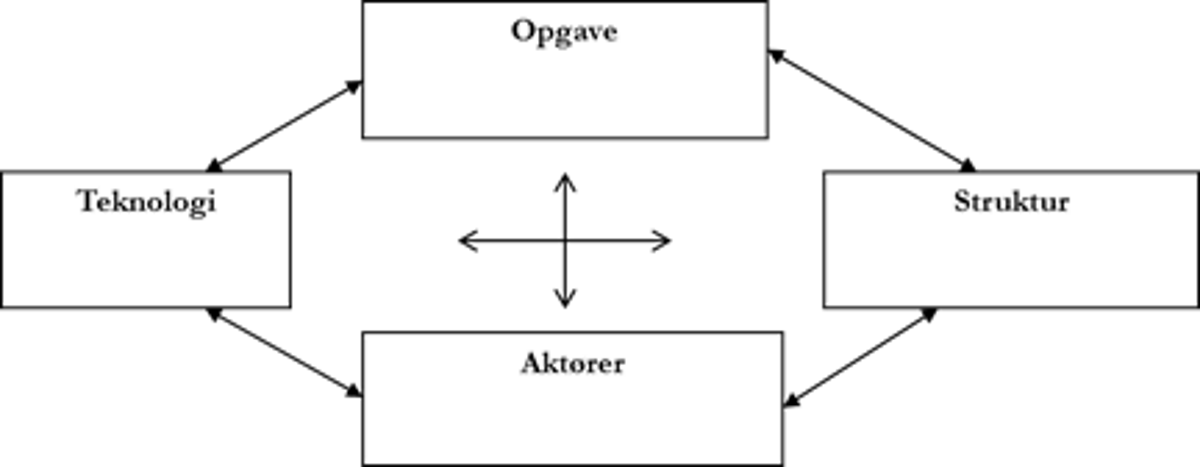
\includegraphics[width = 0.7\textwidth]{Figurer/LeavittModel}
	\caption{Leavitts organisationsmodel, viser hvordan struktur, aktører, opgaver og teknologi indbyrdes relaterer til hinanden \cite{diamantmodel}.}
	\label{DiamantModel}
\end{figure}

Da analysen bygger på dataindsamling fra to kliniske afdelinger, HEH og RMV, vil dens generaliserbarhed potentielt være begrænset. Resultatet heraf kan derfor ikke nødvendigvis anvendes på lignende hospitalsafdelinger i Danmark. 

Dataindsamlingen til analysen er indhentet gennem interview med afdelingssygeplejerske Tina Arnbjørn og tre sonografer fra HEH, samt interview med afdelingssygeplejerske Karen Marie Goul og en sonograf fra RMV.
Til at underbygge problemstillingen omkring arbejdsgener suppleres der med videnskabelige artikler.

\section{HEH}
HEH er bemandet af en afdelingssygeplejerske, fem sonografer samt et ukendt antal læger. Antallet af læger er ikke relevant for denne analyse, da der udelukkende fokuseres på sonografernes arbejdsgange.
Afdelingen har udstyr til fire stuer, hvoraf tre stuer bemandes af sonografer. Der foretages 30-40 scanninger om dagen på afdelingen, og hver scanning tager i gennemsnit 35 minutter. 
Ovenstående information er blevet opsamlet under interview med afdelingssygeplejerske Tina Arnbjørn på HEH, se Bilag 4.

\section{RMV}
Bemanding på RMV består af en afdelingssygeplejerske, ni sonografer og et ukendt antal læger. Afdelingen har ultralydsscanningsudstyr til fem stuer til gravide, hvoraf tre stuer er i drift dagligt og bemandes af sonografer. Dagligt foretages der 25-30 scanninger på afdelingen. En scanning tager i gennemsnittet 30 minutter.
Informationerne for RMV er opnået igennem interview med en sonograf fra afdelingen og afdelingssygeplejerske Karen Marie Goul, se Bilag 5.

\section{Leavitts organisationsmodel}
Det er valgt at sammenskrive de indsamlede data fra HEH og RMV, da afdelingerne er sammenlignelige. Leavitts organisationsmodel vil klarlægge afdelingers organisation og struktur. Derudover vil modellen belyse, hvordan organisationsstrukturen, opgaver og organisationens ansatte bliver påvirket af implementeringen af den nye teknologi \cite{Leavitt} \cite{diamantmodel}. 


\subsection{Opgaver}
Opgaverne som afdelingerne varetager på nuværende tidspunkt vil ikke ændre sig ved implementering af robotarmen, da behovet for scanninger af gravide er uændret. Opgaverne består af nakkefoldsscanning i 11.-13. uge, misdannelsesscanning i 19.-22. uge, vægtscanninger samt diverse kontrolscanninger under graviditeten \cite{graviditet}.

\subsection{Teknologi}
Ved implementering af en ny teknologi, som Ultralyds Robotarmen, sættes der krav til aktørernes faglige kundskaber og erfaringer i brugen af teknologien. Dette er gældende for samtlige sonografer, der skal benytte robotarmen. Der skal derfor være en indkørselsperiode af teknologien førend, den vil være i fuld brug, og før alt personale har kompetencerne til brugen af robotarmen. \\
Det vurderes, at de eksisterende stuer på HEH og RMV er tilstrækkelig store til, at teknologien vil kunne implementeres uden yderligere ændringer. På RMV kan det dog blive nødvendigt at flytte patientskærmen, da robotarmsstativet, se kapitel \ref{Teknologi}, muligvis vil komme til at dække for den gravides udsyn til skærmen.  

\subsection{Aktører} \label{aktoerer_organisation}
Muskel- eller skeletbesvær forårsaget eller forværret af de arbejdsopgaver, som udføres på arbejdspladsen er af typen work-related musculoskeletal disorders (WRMSD). De fremkommer ved gentagne belastninger, kraftkrævende eller akavede bevægelser. I 2008 oplevede op til 90\% af sonograferne smerter under udførelsen af scanninger. Disse smerter kan blive en økonomisk og personlig udgift for den enkelte sonograf i hverdagen \cite{24}\cite{30}\cite{31}\cite{36}.\\
På både HEH og RMV underbygger udtalelser fra sonograferne billedet af, at mange af dem oplever smerter under scanninger. 
Her er den udbredte holdning, at arbejdet er belastende, og der er usikkerhed om, hvor længe den enkelte sonograf kan blive i stillingen. Det belastende arbejde, samt den stigende tendens for kvinders BMI, bidrager til denne usikkerhed \cite{kvinderovervaegt}\cite{24}\cite{31}. \\
Dog er sonograferne positive omkring deres stilling, hvilket kan være med til at undertrykke eventuelle smerter, sådan at sonografen kan forblive længere tid i sin stilling \cite{1}\cite{24}.

WRMSD og smerter ses i nakke, skulder og håndled, og kan forekomme af drejende bevægelser i nakke og krop, håndledsbøjninger og arbejde i udstrakt arm. Smerterne kan også stamme fra inflammation af senerne i hånd og håndled, hvilke forekommer af belastningen fra grebet om ultralydsproben sammen med håndledsbøjninger \cite{24}\cite{31}\cite{32}\cite{36}. Se figur \ref{wrist} og \ref{udstraktArm}.

\begin{figure}[H]
  \begin{minipage}{0.49\textwidth}
    \centering
      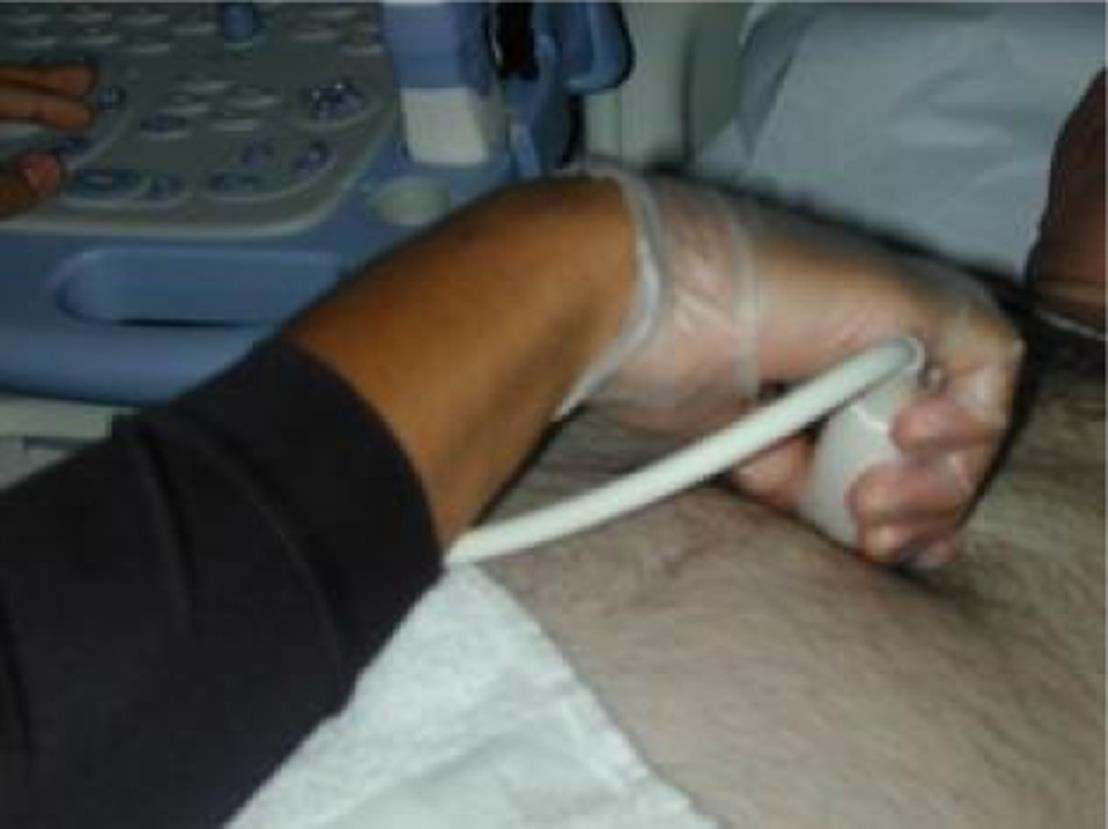
\includegraphics[width=\textwidth]{Figurer/wrist.jpg}
      \caption{Håndledsbøjning og greb om proben \cite{31}}
    \label{wrist}
  \end{minipage}
  \hspace{0.02\textwidth}
  \begin{minipage}{0.47\textwidth}
    \centering
      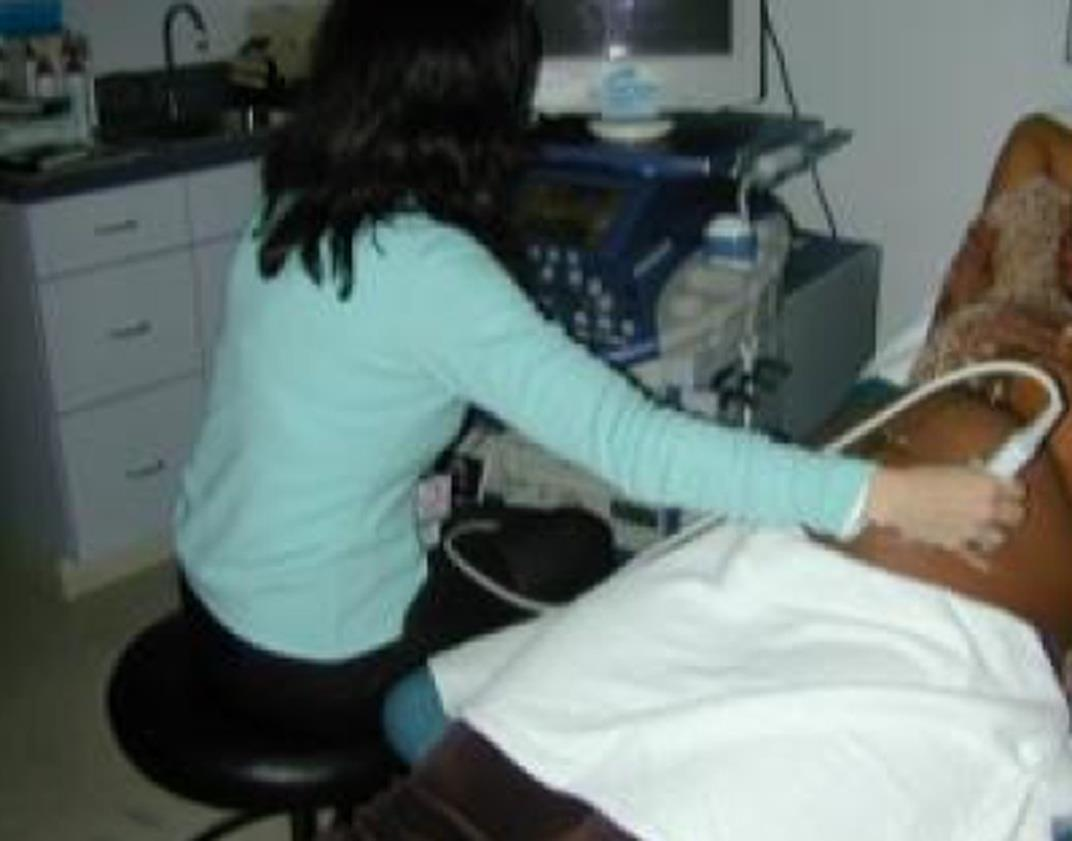
\includegraphics[width=\textwidth]{Figurer/arm.jpg}
      \caption{Arbejde i udstrakt arm \cite{31}}
    \label{udstraktArm}
  \end{minipage}
\end{figure}

Implementeringen af robotarmen vil føre til markante ændringer for sonografernes arbejdsstillinger. Disse ændringer sker idet, sonografen ikke længere skal sidde med udstrakt arm ind over den gravide, og skaderne i skulderen vil derfor kunne undgås. Desuden vil sonografen være mere centreret omkring arbejdsstationen og derfor vil vrid i kroppen og nakken også blive mindsket. Sonografen skal stadig holde om dummy-proben, se kapitel \ref{Teknologi}, så den gribende belastning kan ikke fjernes helt. Da de resterende belastninger kan mindskes eller helt fjernes, vil dette ikke have den samme belastende virkning. 

En undersøgelse er blevet udført af Robotic Ultrasound ApS for at efterprøve, hvor mange kilo sonograferne skal påtrykke proben med under en ultralydsscanning. Her blev proben påført et dynamometer, hvilken måler trykket sonografen påtrykker med under en scanning. Resultatet heraf blev, at sonograferne ved de almindelige og ukomplicerede scanninger, som en nakkefoldsscanning, trykker med 2-3 kg. Sonograferne skal trykke med omkring 11 kg ved de mere komplicerede scanninger, som scanning på gravide med bagoverbøjet livmoder \cite{livmoder}. Trykket føles dog større for sonografen, da trykket skal påføres i udstrakt arm. Undersøgelsen blev udført på 5 sonografer over én arbejdsdag, se Bilag 12, 28.04.2016.

Den generelle holdning på HEH og RMV er meget teknologivenlig. Derfor formodes det, at implementeringen af teknologien ikke vil føre til væsentlige problemer i forhold til at få sonograferne til at benytte Ultralyds Robotarmen. Implementeringen kræver dog, at der tilrettelægges en ordentlig plan for oplæring af sonograferne i brugen af teknologien. Sonograferne har generelt en god holdning og tillid til teknologi og er åbne for en mulig implementering af Ultralyds Robotarmen.

\subsection{Struktur}
Pr. juni 2016 er den strukturelle opbygning på afdelingerne således, at en medarbejder ultralydsscanner henholdsvis 30 timer på HEH og 22 timer på RMV om ugen. De resterende timer udmønter sig som aflastende arbejde for den enkelte medarbejder. Denne struktur skyldes, at det er et kendt problem på afdelingerne, at scanningsarbejdet er fysisk belastende for medarbejderen. I løbet af en scanningsdag har én medarbejder i gennemsnit ti scanninger. Yderligere foretages der på afdelingerne forebyggende tiltag i form af styrketrænende elastikøvelser, mulighed for gratis massage, ergonomiske redskaber samt fri adgang til fysioterapeuter og wellness-konsulenter, der kontrollerer og vejleder om medarbejderens arbejdsstillinger, se Bilag 4 og Bilag 5.

Afdelingerne tilrettelægger selv mængden af tid den enkelte sonograf skal scanne i løbet af en uge. Dansk Føtalmedicinsk Selskab udstikker hvert femte år anbefalinger, som afdelingerne tilrådes at følge. Anbefalingerne i forhold til antal timers ultralydscanning er 28 timer pr. uge, da det er vurderet, at ved denne mængde af scanninger vil belastningen af sonografen ikke være i en skadende grad, se Bilag 10. Denne vurdering underbygges af videnskabelige forskningsundersøgelser, hvor sonografernes arbejdsskader og mængden af scanningstid er blevet sammenholdt. Disse undersøgelser viser yderligere, at en arbejdsskade typisk optræder efter 5 års arbejde, hvilket der skal tages højde for i valget af observationsgruppe til lignende undersøgelser \cite{35}.

Ud fra dette bemærkes det, at RMV arbejder 6 timer under anbefalingerne, mens sonograferne på HEH scanner to timer mere om ugen end anbefalet. Årsagerne hertil kan være flere. En typisk årsag vil være, at normeringerne og bevillingerne til antal af sonografer og antallet af scanninger, ikke gør det muligt at tilpasse arbejdsforholdet til anbefalingerne. 

Implementering af robotarmen vil føre til en ændring i afdelingernes strukturelle opbygning. Ultralyds Robotarmen vil gøre scanningsarbejdet væsentlig mindre belastende, og dermed vil det kunne føre til, at en medarbejder vil kunne scanne på fuldtidsbasis, altså 37 timer om ugen. Arbejdsstillingerne, som sonograferne udfører, og hvordan disse vil ændre sig, er beskrevet i afsnittet \ref{aktoerer_organisation}. Hvis sonograferne scanner 37 timer om ugen, vil opgaverne de varetager som aflastende arbejde, herunder bl.a. fostervandsprøver, se Bilag 4, og medicinske aborter, se Bilag 5, kunne blive varetaget af andet personale. Yderligere kan det føre til en ændring i antallet af sonografer, der er behov for på den enkelte afdeling. 

HEH har på nuværende tidspunkt indvilliget i at være testafdeling for Robotic Ultrasound ApS under udviklingen og test af produktet. Det er i afdelingens interesse, da der ses en fremtid i produktet. Det ønskes fra afdelingens side at være med under tilpasningen af produktet til afdelingens struktur og behov. 

\section{Delkonklusion}
Organisatorisk vil implementering af Ultralyds Robotarmen kunne føre til færre arbejdsgener blandt sonografer. Samtidig vil brugen af robotarmen ikke skabe store ændringer i den daglige arbejdsgang, samt den strukturelle opbygning på den enkelte afdeling. \\
Det vurderes, at ved færre arbejdsgener vil mængden af scanningstimer pr. sonograf kunne hæves til 37 timer om ugen. Dette vil dermed på sigt kunne føre til at behovet for antallet af sonografer vil falde.

Begge de adspurgte afdelinger HEH og RMV er åbne for indførslen af robotarmen som en ny teknologi, og dermed ses dette ikke som en begrænsning. Yderligere er de eksisterende stuer af en tilstrækkelig størrelse til at robotarmen vil kunne implementeres uden behov for store udvidelser. 